Um ein Bild von der allgemeinen Übereinstimmung der simulierten Daten mit den tatsächlich beobachteten Daten zu erhalten wird in diesem Kapitel das Jahresmittel der simulierten und beobachteten Daten verglichen. Dadurch erhält man einen Überblick über die geographische Übereinstimmung der Regenzonen und Trockengebiete im abgebildeten Bereich.\\
Die Berechnungen erfolgten im wesentlichen folgendem Schema:
\begin{enumerate}
	\item Berechnung des jährlichen Mittelwertes pro Gitterzelle über aller Jahre
	\item Subtraktion dies Mittelwerte (Simuliert - Beobachtet)
	\subitem[a] Mittelwerte pro Gitterzelle über die Differenzen
	\subitem[b] 90. und 99. Quantil der jährlichen Differenzen der Mittelwerte
\end{enumerate}
\section{EUR-11 Datensatz}
In diesem Unterkapitel wird ausschließlich der EUR-11 Datensatz evaluiert, welcher ganz Europa abbildet. Der Beobachtungsdatensatz ist E-OBS\cite{eobs}.\\
\begin{figure}[hbt!]
	\begin{subfigure}{0.49\textwidth}
		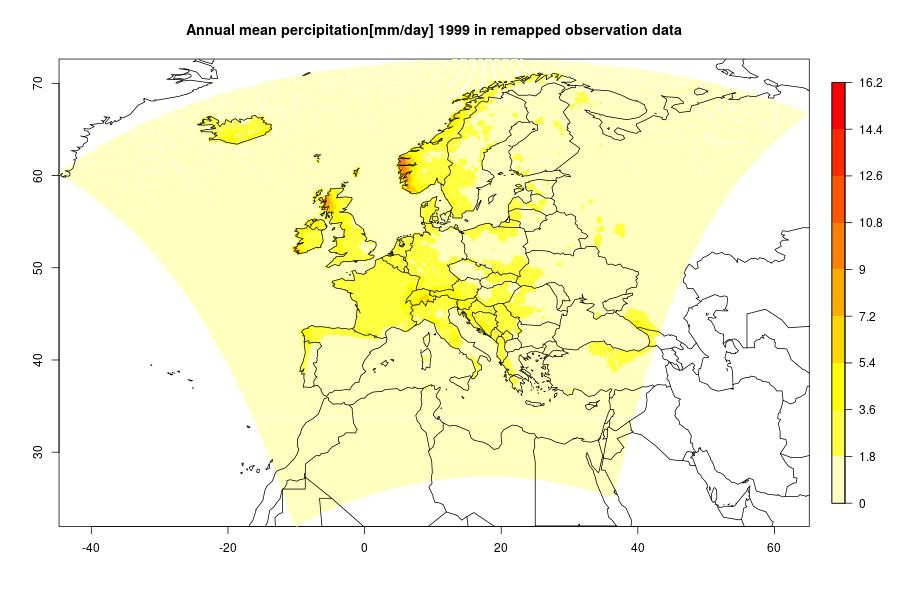
\includegraphics[width=\textwidth]{mean/mprs1999obs_remapped.jpg}
		\caption{Jährliches Mittel über den Niederschlag im Jahr 1999 der tatsächlich Beobachteten Daten}
		\label{fig:mobs99}
	\end{subfigure}
	\begin{subfigure}{0.49\textwidth}
		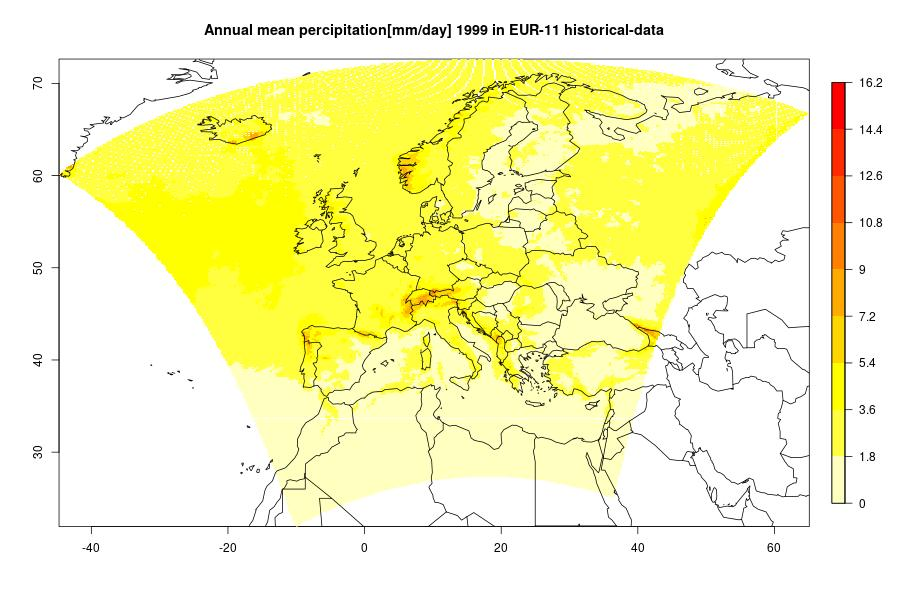
\includegraphics[width=\textwidth]{mean/msim1999hist.jpg}
		\caption{Jährliches Mittel über den Niederschlag im Jahr 1999 im historical Datensatz von EUR-11}
		\label{fig:mhist99}
	\end{subfigure}
	\begin{subfigure}{\textwidth}
		\centering
		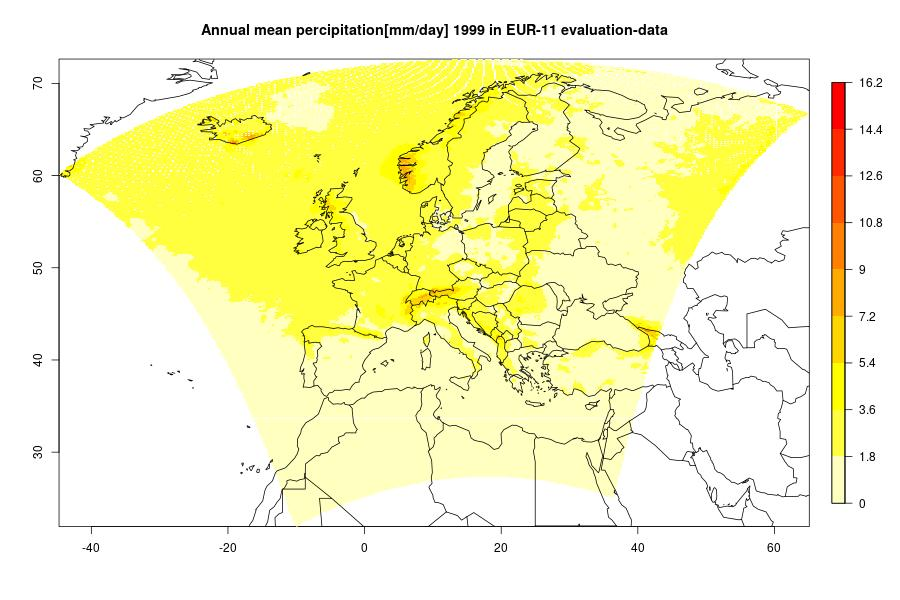
\includegraphics[width=\textwidth]{mean/msim1999eval.jpg}
		\caption{Jährliches Mittel über den Niederschlag im Jahr 1999 im evaluation Datensatz von EUR-11}
		\label{fig:meval99}
	\end{subfigure}
	\caption{Jährliches Mittel über den Niederschlag im EUR-11 Datensatz für das Jahr 1999}
\end{figure}
\\
Zu Abb. \ref{fig:mobs99}: Man erkennt gut die starken Regenfälle an der Westküste Norwegens und Englands (bis zu 12.6 mm). Der Niederschlag an Irlands Westküste und im Alpenbereich fielen 1999 im Mittel schwach aus (bis zu 7.2mm). Über Deutschland, Frankreich und weiten Teilen Europas fielen im Schnitt 3.6-5.4 mm Regen am Tag.\\
\\
Zu Abb. \ref{fig:mhist99}: Der Regen an der norwegischen Westküste fällt bei dieser Modellaufnahme um einiges schwächer aus als in der Aufnahme des Evaluation Datensatzes zuvor. Dies ist noch auffallender im Vergleich mit den Beobachtungsdaten. Mit dem Niederschlag an der britischen Westküste verhält es sich ähnlich, Auffallend sind besonders die Erscheinungen im Süden Frankreichs, wo aus unersichtlichen Gründen im Flachland um Toulouse größere Regenmengen \glqq voraus \grqq-gesagt wurden. Die Analyse des Alpenraums und des Kaukasusgebiets fallen fast gleich aus wie die im Evaluationsdatensatz (Abb. \ref{fig:meval99}). Bei dieser Herangehensweise wurde das CCLM mit dem GCM MPI-ESM-LR für die historische Periode 1999 angetrieben. Es sind darin wohl einige Abweichungen zum tatsächlichen Globalen Klima vorhanden, aber auch das downscaling hat diese Abweichungen hervorgebracht. Dies wird im nächsten Unterkapitel beim Vergleichen mit den Ergebnissen einer konvektionserlaubenden Simulation (ALP-3 Daten) ersichtlich.\\
\begin{figure}[hbt!]
	\centering
	\begin{subfigure}{0.49\textwidth}
		\centering
		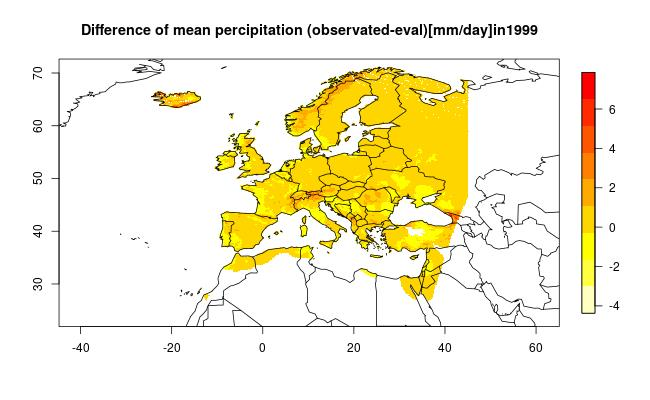
\includegraphics[width=\textwidth]{mean/1999dif_mprs_eval-obs.jpg}
		\caption{Differenz des Beobachtungsdatensatzes und des evaluation-Datensatzes}
		\label{fig:eval_dif}
	\end{subfigure}
	\begin{subfigure}{0.49\textwidth}
		\centering
		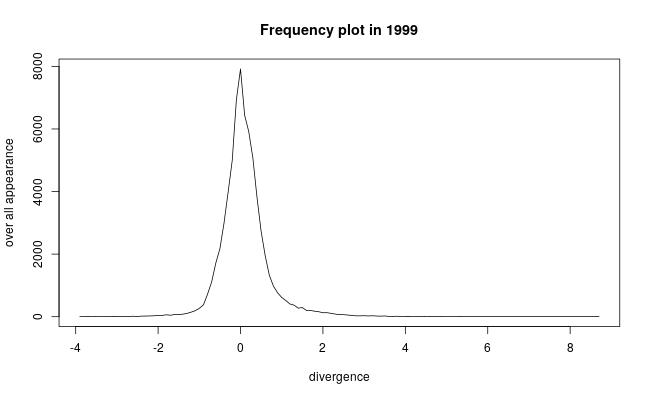
\includegraphics[width=\textwidth]{mean/1999frequenciesdif_mprs_eval-obs.jpg}
		\caption{Häufigkeit der Abweichungen über das gesamte Gitter}
		\label{fig:eval_freq_dif}
	\end{subfigure}
	\begin{subfigure}{0.49\textwidth}
		\centering
		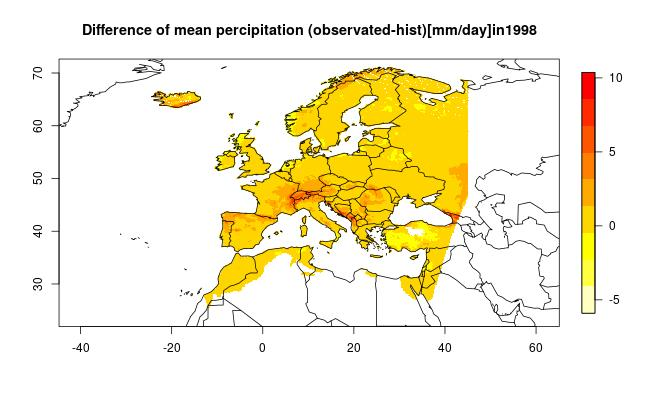
\includegraphics[width=\textwidth]{mean/1999dif_mprs_hist-obs.jpg}
		\caption{Differenz des Beobachtungsdatensatzes und des historical-Datensatzes}
		\label{fig:hist_dif}
	\end{subfigure}
	\begin{subfigure}{0.49\textwidth}
		\centering
		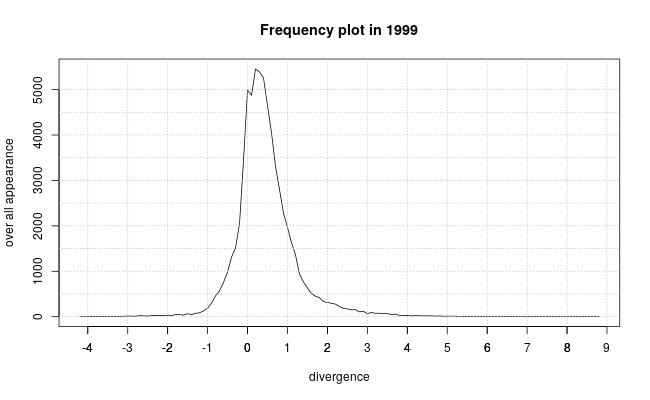
\includegraphics[width=\textwidth]{mean/1999frequenciesdif_mprs_hist-obs.jpg}
		\caption{Häufigkeit der Abweichungen über das gesamte Gitter für den historical-Datensatz}
		\label{fig:hist_freq_dif}
	\end{subfigure}
	\caption{Differenzen für den evaluation- und historical- Datensatz im Jahr 1999}
\end{figure}
\\
Wie man gut in Abb. \ref{fig:eval_dif} erkennen kann ist im allgemeinen über den orthographisch gediegenen Gegenden die Abweichung vom Beobachtungsdatensatz gering. Es ist gut ersichtlich, dass die Abweichungen in überwiegend gebirgigen Gegenden größer sind. Wie auch in Abb. \ref{fig:eval_freq_dif} zu sehen ist, überwiegt eine Abweichung von 0, auch wenn die Kurve leicht ins rechte verschoben ist - dies bedeutet dass mehr Niederschlage simuliert wurde als es tatsächlich gab. Der Mittelwert der Abweichungen in diesem Datensatz beträgt für das Jahr 1999 $+0.1009$.\\
Man kann auch gut erkennen, dass im historical-Datensatz (siehe Abb. \ref{fig:hist_dif}) die Abweichungen größer sind als im evaluation Datensatz, was darauf zurückzuführen ist, dass für den historical-Datensatz die Auswirkungen eines simulierten globalen Klimas auf regionale Ebene berechnet wurden, und dadurch Abweichungen zur tatsächlichen Konstellation der Atmosphäre von vorneherein herrschen. Der Mittelwert der Abweichungen in diesem Datensatz beträgt für das Jahr 1999 $+0.4590$. Dies ist bedeutend höher als im evaluation-Datensatz. Man kann dies auch gut in der Abbildung \ref{fig:hist_freq_dif} erkennen, wo die maximale Häufigkeit nicht mehr über $0$ sondern über ca. $+0.3$ liegt.\\
Im folgenden sollen alle Jahre gemittelt verglichen werden um eine Allgemeinaussage über das GCM MPI-ESM-LR und das betreffende CCLM4-8-17 treffen zu können:\\
\begin{figure}[hbt!]
	\begin{subfigure}{0.49\textwidth}
	\centering
	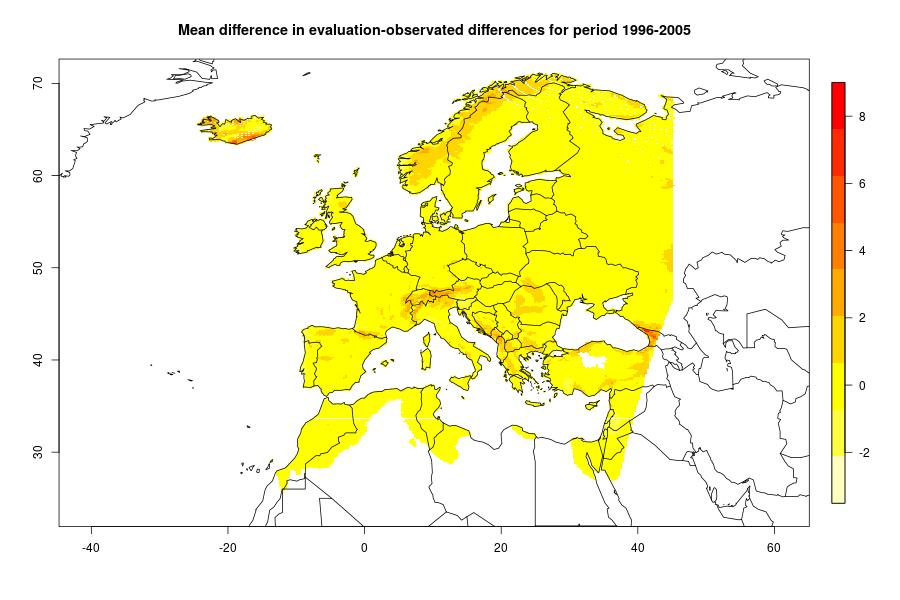
\includegraphics[width=\textwidth]{mean/dif_mean_eval.jpg}
	\caption{Gemittelte Abweichungen von den Beobachtungsdaten über die gesamte Periode für den EUR-11 Evaluations-Datensatz}
	\label{fig:mean_dif_eval}
	\end{subfigure}
	\begin{subfigure}{0.49\textwidth}
		\centering
		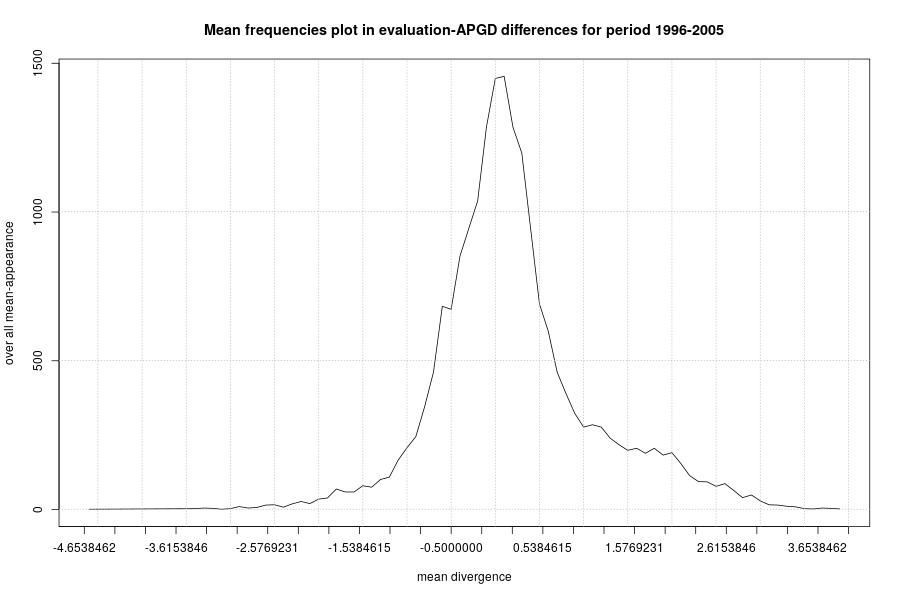
\includegraphics[width=\textwidth]{mean/frequenciesdif_mean_eval.jpg}
		\caption{Gemittelte Häufigkeit der Abweichungen von den Beobachtungsdaten über die gesamte Periode für den EUR-11 Evaluations-Datensatz}
		\label{fig:freq_mean_dif_eval}
	\end{subfigure}
	\begin{subfigure}{0.49\textwidth}
	\centering
	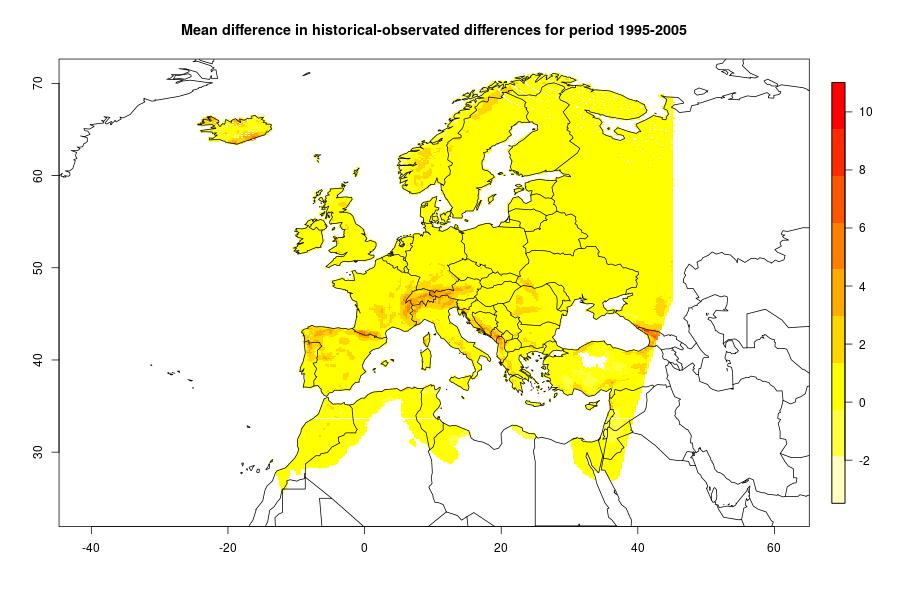
\includegraphics[width=\textwidth]{mean/dif_mean_hist.jpg}
	\caption{Gemittelte Abweichungen von den Beobachtungsdaten über die gesamte Periode für den EUR-11 historical-Datensatz}
	\label{fig:mean_dif_hist}
	\end{subfigure}
	\begin{subfigure}{0.49\textwidth}
			\centering
		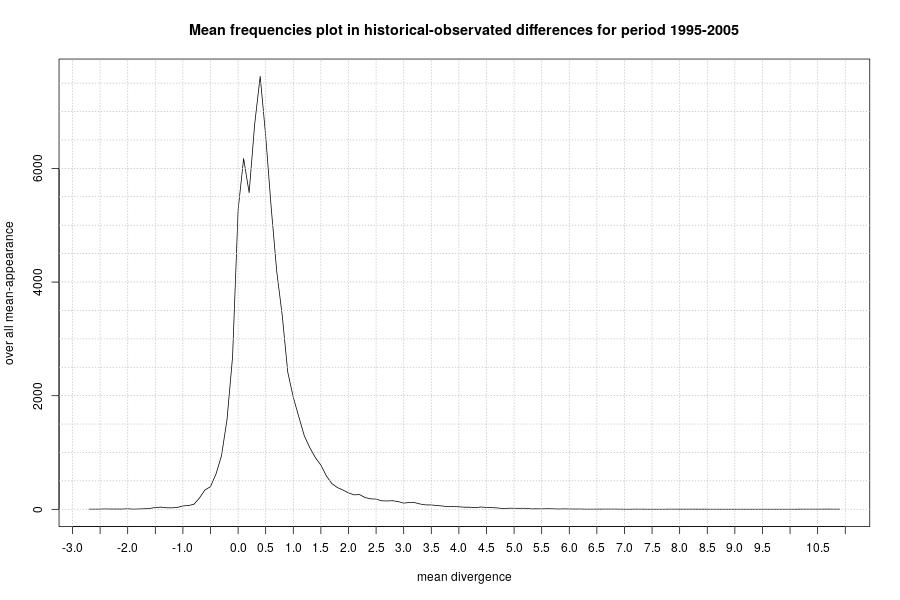
\includegraphics[width=\textwidth]{mean/frequenciesdif_mean_hist.jpg}
		\caption{Gemittelte Häufigkeit der Abweichungen von den Beobachtungsdaten über die gesamte Periode für den EUR-11  historical-Datensatz}
		\label{fig:freq_mean_dif_hist}
	\end{subfigure}
	\caption{Gemittelte Abweichungen im EUR-11 Datensatz}
\end{figure}
\\
Die Differenzen vom historical-Datensatz zu den Beobachtungsdaten, die wir zuvor für das Jahr 1999 zeigen konnten, scheint sich im Mittel auch für die gesamte Periode 1995-2005 abzubilden. Man erkennt beim vergleichen der Abb. \ref{fig:mean_dif_hist} und \ref{fig:hist_dif}, dass sich der Mittelwert in der Verteilungskurve noch weiter ins positive verschoben hat. Man erhält eine mittlere Abweichung von $0.5568$. Somit wurde auch gemittelt zu viel Niederschlag simuliert.\\
Auch die mittleren Abweichungen im evaluation-Datensatz sind ähnlich, es zeichnet sich dasselbe Muster wie im Jahre 1999 ab. Wobei auch hier, wie im historical-Datenatz der Durchschnitt leicht ins Positive verschoben ist(vgl. dazu Abb.\ref{fig:freq_mean_dif_eval} und Abb.\ref{fig:eval_freq_dif}): die höchste Häufigkeit liegt zwar immer noch über $0$ aber die mittlere Abweichung liegt bei $0.1297$ was um $0.0289$ über der des Jahres 1999 liegt. Somit entspricht das über die gesamte Periode gemittelte Maß für den Niederschlag noch weniger dem Beobachteten Werten.\\
Wie in den Abbildungen \ref{fig:q90_dif_eval} und \ref{fig:q90_dif_hist} zu erkennen ist, herrscht die größte Abweichung in den Gebirgen (Südküste Islands, Westküste Norwegens, Alpen ,Pyrenäen, Kantabrisches Gebirge und Kaukasus) jedoch reicht auch dort das 90. Quantil nicht weit über 10mm/Tag hinaus (siehe Abb.\ref{fig:q90_freq_dif_eval} und Abb.\ref{fig:q90_freq_dif_hist}), was eine einigermaßen gute Übereinstimmung mit der beobachteten Wetterlage auszeichnet. Im Mittel wurden dementsprechend maximal 10mm zu viel simuliert, was der fehlenden Simulation der Konvektion zuzuschreiben ist, wir werden im folgenden Kapitel sehen, dass die Abweichung weitaus geringer ausfällt, wenn diese simuliert wird. \\
\begin{figure}[hbt!]
	\begin{subfigure}{0.49\textwidth}
		\centering
		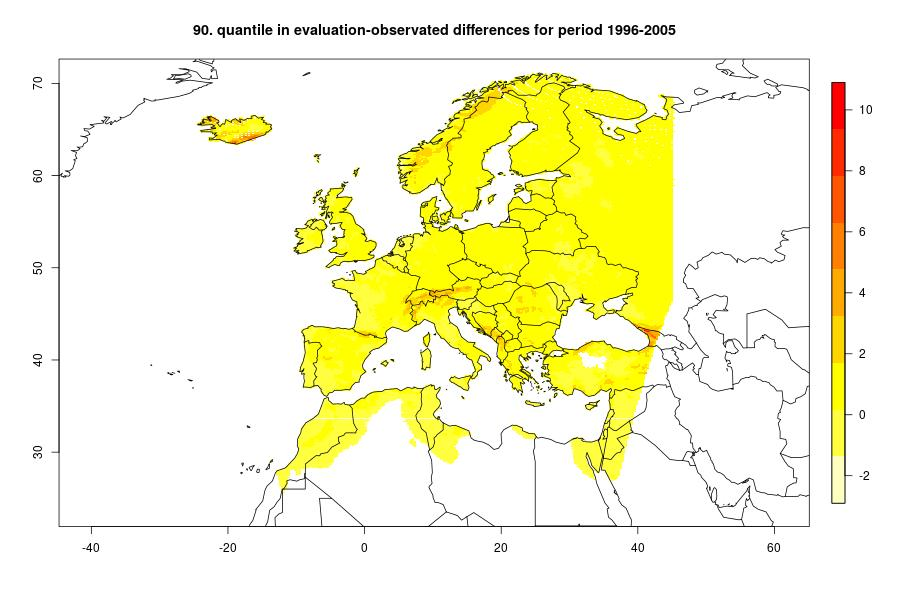
\includegraphics[width=\textwidth]{mean/dif_q90_eval.jpg}
		\caption{90. Quantil der Abweichungen von den Beobachtungsdaten über die gesamte Periode für den EUR-11 evaluation-Datensatz}
		\label{fig:q90_dif_eval}
	\end{subfigure}
	\begin{subfigure}{0.49\textwidth}
		\centering
		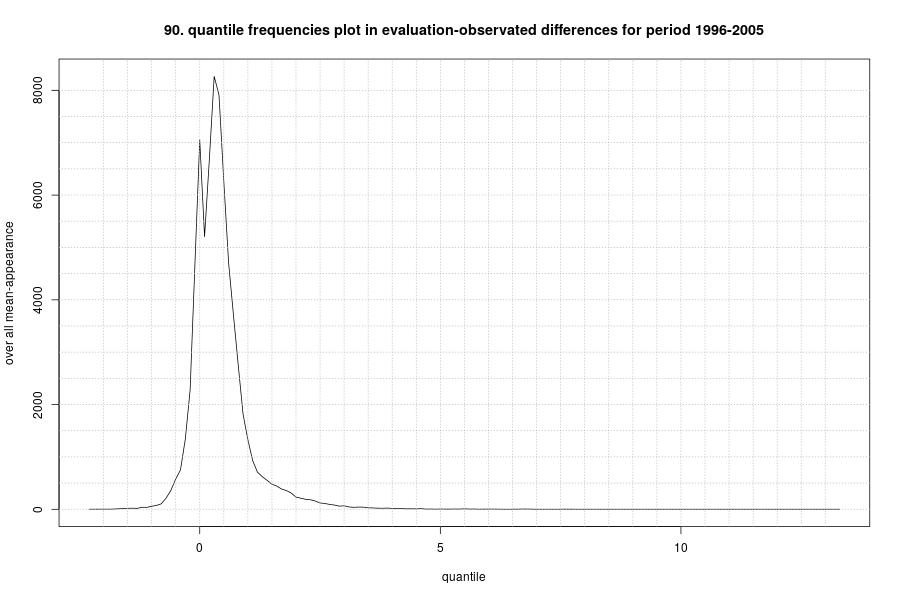
\includegraphics[width=\textwidth]{mean/frequenciesdif_q90_eval.jpg}
		\caption{Häufigkeit des 90. Quantil in der Abweichungen von den Beobachtungsdaten über die gesamte Periode für den EUR-11 evaluation-Datensatz}
		\label{fig:q90_freq_dif_eval}
	\end{subfigure}
	\begin{subfigure}{0.49\textwidth}
		\centering
		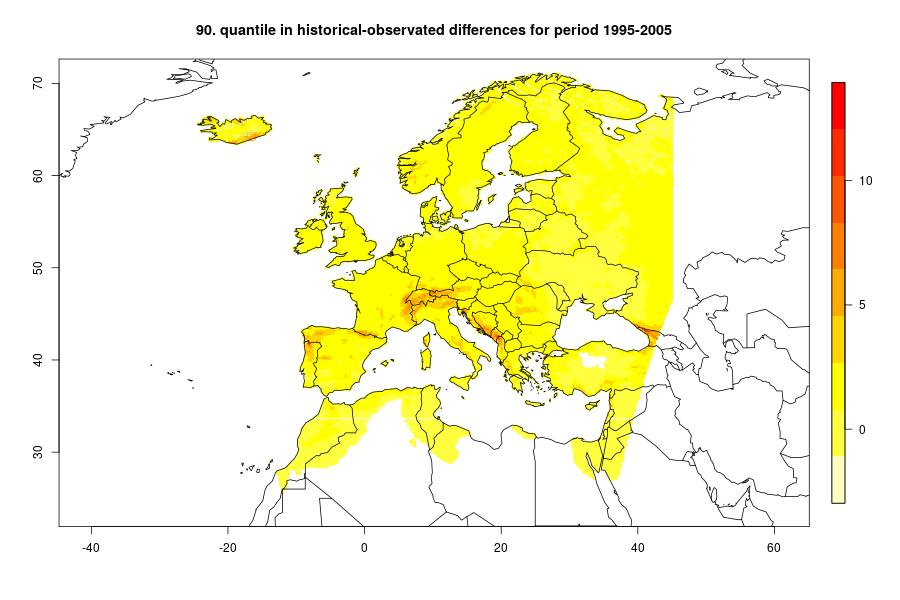
\includegraphics[width=\textwidth]{mean/dif_q90_hist.jpg}
		\caption{90. Quantil der Abweichungen von den Beobachtungsdaten über die gesamte Periode für den EUR-11 historical-Datensatz}
		\label{fig:q90_dif_hist}
	\end{subfigure}
	\begin{subfigure}{0.49\textwidth}
		\centering
		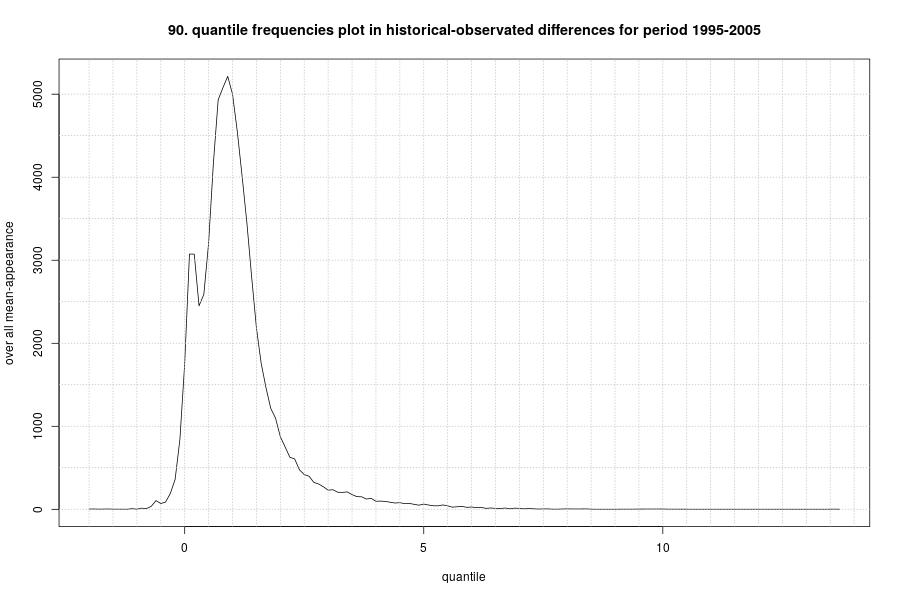
\includegraphics[width=\textwidth]{mean/frequenciesdif_q90_hist.jpg}
		\caption{Häufigkeit des 90. Quantil in der Abweichungen von den Beobachtungsdaten über die gesamte Periode für den EUR-11 historical-Datensatz}
		\label{fig:q90_freq_dif_hist}
	\end{subfigure}
	\caption{90. Quantil der mittleren Abweichungen im EUR-11 Datensatz}
\end{figure}
\\
\pagebreak

\section{ALP-3 - Datensatz}
In diesem Unterkapitel wird ausschließlich der ALP-3 Datensatz mit dem APGD -Datensatz von MeteoSwiss \cite{apgd} verglichen. Dieser Datensatz bildet den Alpenraum und nordöstlichen Bereich des Mittelmeers ab, die APGD Daten reichen wie weiter unten ersichtlich nicht über den gesamten Bereich, die Vergleichsberechnungen ziehen natürlich nur die von beiden Datensätzen abgedeckten Flächen in Betracht.\\
\begin{figure}[hbt!]
	\begin{subfigure}{0.49\textwidth}
	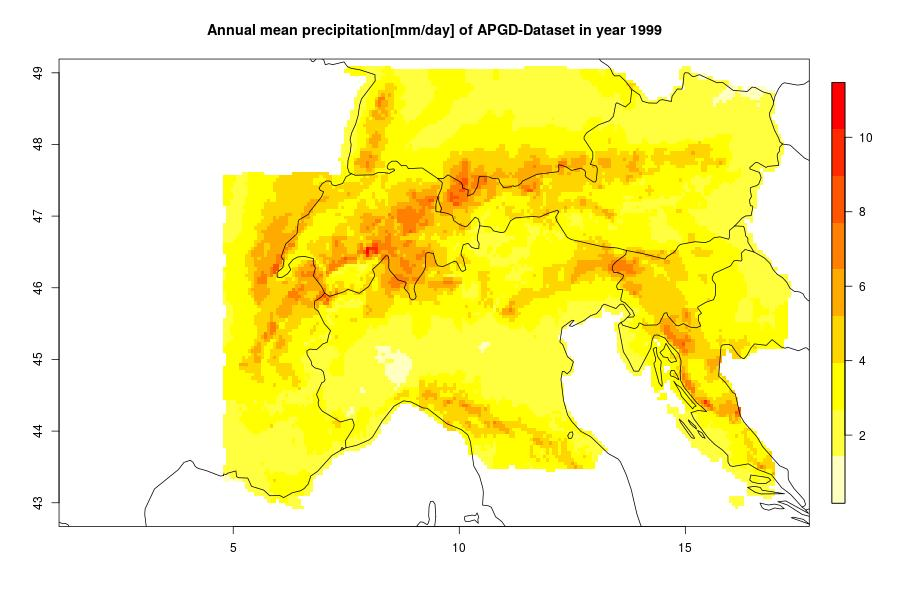
\includegraphics[width=\textwidth]{mean/ALP3/mprs-apgd-1999.jpg}
	\caption{Jährliches Mittel des Niederschlags im Jahr 1999 aus dem Beobachtungsdatensatz(APGD)}
	\label{fig:mean_apgd_1999}
	\end{subfigure}
	\begin{subfigure}{0.49\textwidth}
		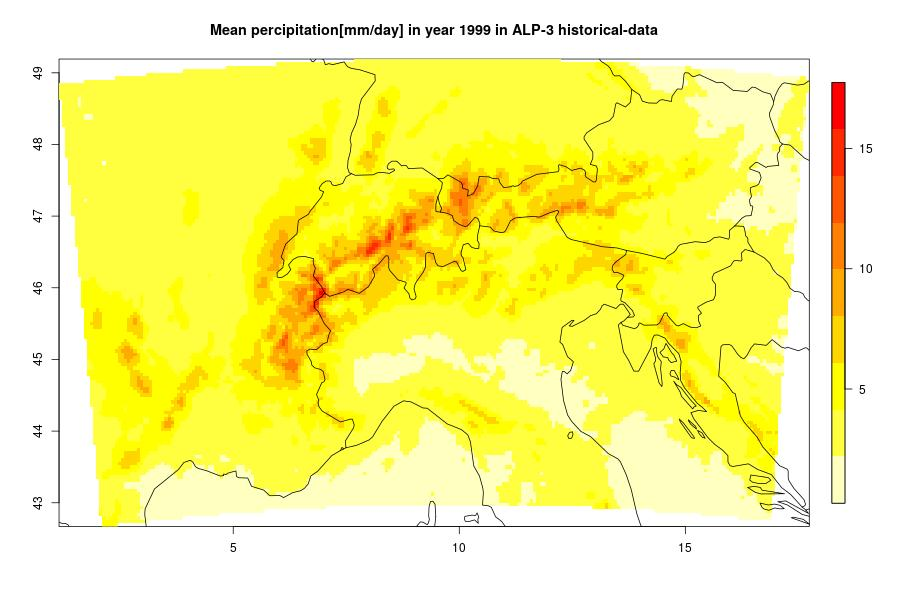
\includegraphics[width=\textwidth]{mean/ALP3/mprs-1999historical-alp3.jpg}
		\caption{Jährliches Mittel des Niederschlags im Jahr 1999 aus den historical-Daten im ALP-3}
		\label{fig:mean_hist_alp3_1999}
	\end{subfigure}
	\begin{subfigure}{0.49\textwidth}
		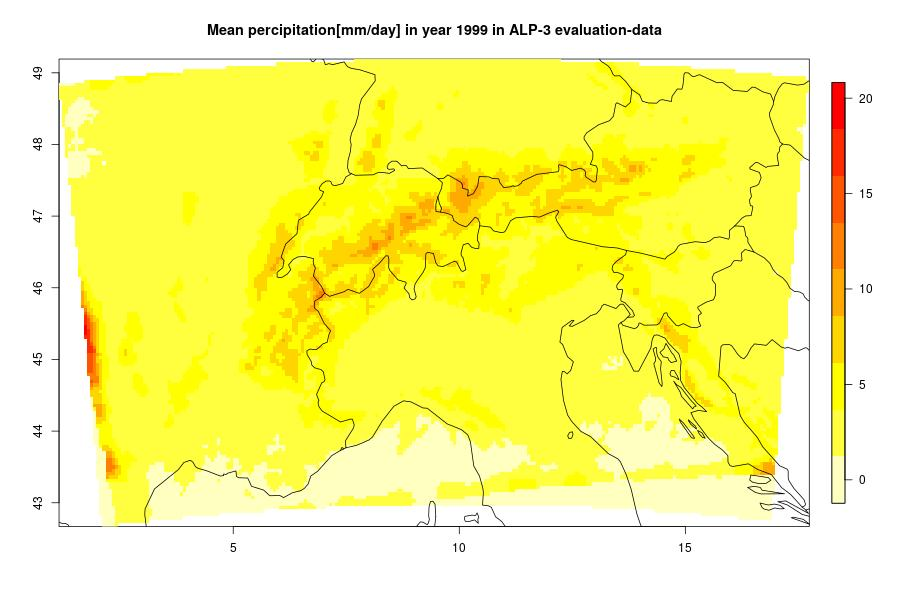
\includegraphics[width=\textwidth]{mean/ALP3/mprs-1999evaluation-alp3.jpg}
		\caption{Darstellung mit dem Bereich der Ausreißer-Daten}
		\label{fig:mean_eval_alp3_1999}
	\end{subfigure}
	\begin{subfigure}{0.49\textwidth}
		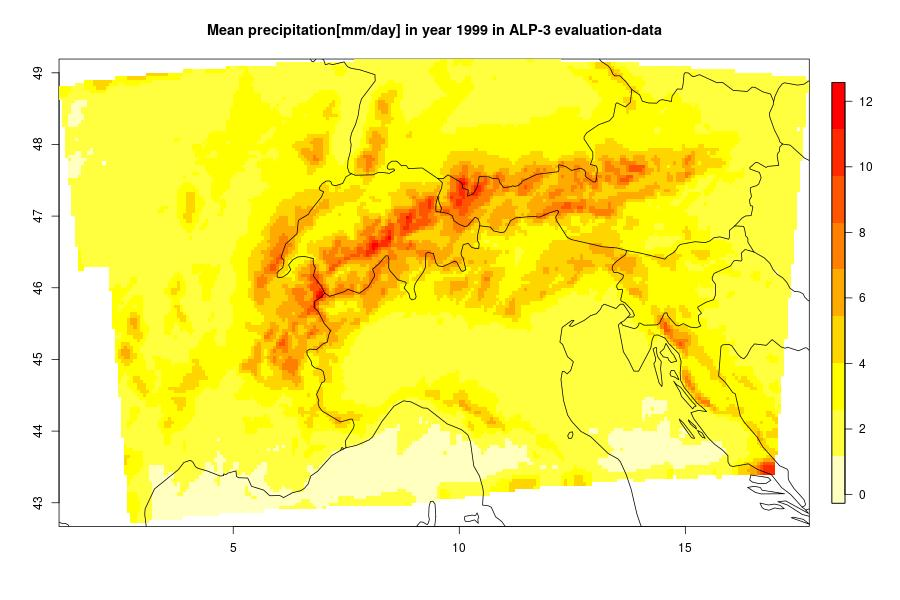
\includegraphics[width=\textwidth]{mean/ALP3/cropped-mprs-1999evaluation-alp3.jpg}
		\caption{Darstellung mit ausgeschnittenem Ausreißer-Bereich}
		\label{fig:cropped_mean_eval_alp3_1999}
	\end{subfigure}
	\caption{Jährliches Mittel des Niederschlags im Jahr 1999}
\end{figure}
\\
Zu Abb. \ref{fig:mean_apgd_1999}: Man erkennt gut die typisch hohen Niederschläge über dem Alpenhauptkamm, besonders ausgeprägt ist auch eine langgezogen Nord-Süd Regenzone über Kroatien und Slowenien sowie auch relativ hohe Niederschläge im unteren Murtal bei Graz.\\
\\
Zu Abb. \ref{fig:mean_hist_alp3_1999}: Hier sind die Niederschlagsmengen etwas größer, jedoch die generellen Niederschlagsmuster am Alpenhauptkamm und über Kroatien werden im historical-Datensatz gut abgebildet, einzig die Niederschläge im unteren Murtal scheinen nicht abgebildet zu sein.\\
\\
Zu Abb. \ref{fig:mean_eval_alp3_1999}: Man sieht, dass die höchsten Niederschläge hier am linken Rand des Gitters stehen, was einen Ausreißer-Wert darstellt, da es sich um sehr lokale überdurchschnittliche Höchstwerte handelt wurden sie ausgeschnitten um eine bessere Darstellung der Werte zu sichern. Die verbesserte Abbildung[\ref{fig:cropped_mean_eval_alp3_1999}] zeigt eine starke Korrelation mit den Beobachtungsdaten, selbst die stärkeren Niederschläge im unteren Murtal wurden mit-simuliert was eine gute allgemeine Übereinstimmung des CCM's verspricht.\\\
Anmerkung: der ausgeschnittene Bereich wird in den folgenden Berechnungen nicht mit einbezogen, da der Datensatz von APGD nicht so weit in den Westen reicht wie die Simulationsdaten.\\
Wie für den EUR-11 Datensatz werden die durchschnittlichen Niederschläge aus dem Jahr 1999 der Beobachtungsdaten von den Simulierten abgezogen um die Differenz abbilden zu können:\\
\begin{figure}[hbt!]
	\begin{subfigure}{0.49\textwidth}
		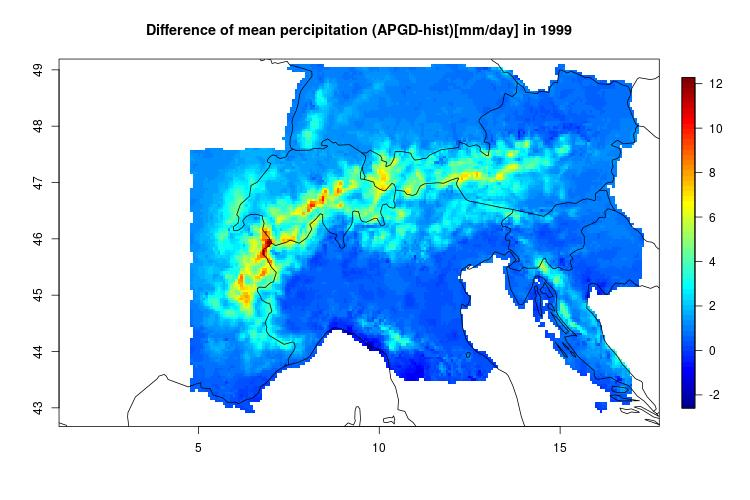
\includegraphics[width=\textwidth]{mean/ALP3/1999dif_mprs_alp3hist-apgd.jpg}
		\caption{Gemittelte Differenz im Jahr 1999 [mm/day] von den historical und APGD Daten}
		\label{fig:dif_hist_apgd_1999}
	\end{subfigure}
	\begin{subfigure}{0.49\textwidth}
		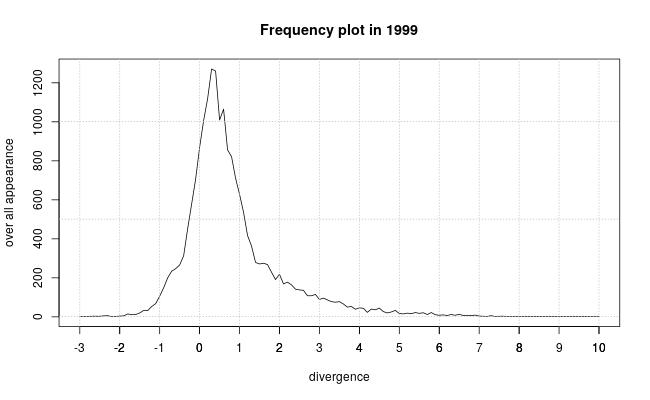
\includegraphics[width=\textwidth]{mean/ALP3/1999frequenciesdif_mprs_alp3hist-apgd.jpg}
		\caption{Absolute Häufigkeit der jährlich gemittelten Differenzen über das gesamt Gitter für das Jahr 1999 [mm/day]}
		\label{fig:freq_dif_hist_apgd_1999}
	\end{subfigure}
	\caption{Jährlich gemittelte Differenzen des Niederschlags im Jahr 1999 der historical Daten mit den APGD-Daten}
\end{figure}
\\
Wie man in Abb. \ref{fig:dif_hist_apgd_1999} gut erkennen kann, ist die Abweichung im Alpenraum überdurchschnittlich hoch, sogar höher als beim vergleichbaren EUR-11 Szenario (siehe Abb. \ref{fig:hist_dif}). Die mittlere Abweichung beträgt hier $+0.8304$ verglichen mit der mittleren Abweichung von $+0.4590$ ist dies eine starke Zunahme. Durch den Vergleich mit den guten Ergebnissen der Berechnungen im evaluation-Datensatz, bestätigt dies die oben getroffene Annahme, dass das GCM MPI-ESM-LR einige Fehler bzw. Abweichungen enthält, was dem CCLM4-8-17 unzureichend genauen Input liefert und es nicht auf Fehler im downscaling selbst beruht.\\
\begin{figure}[hbt!]
	\begin{subfigure}{0.49\textwidth}
		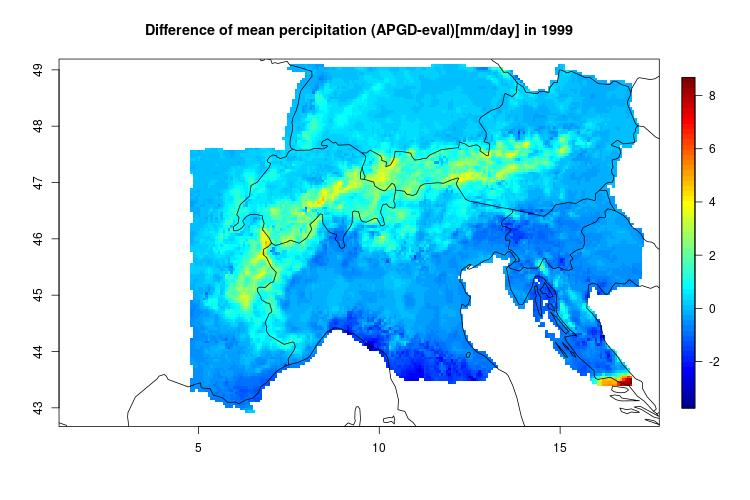
\includegraphics[width=\textwidth]{mean/ALP3/1999dif_mprs_alp3eval-apgd.jpg}
		\caption{Gemittelte Differenz im Jahr 1999 [mm/day] von den evaluation und APGD Daten}
		\label{fig:dif_eval_apgd_1999}
	\end{subfigure}
	\begin{subfigure}{0.49\textwidth}
		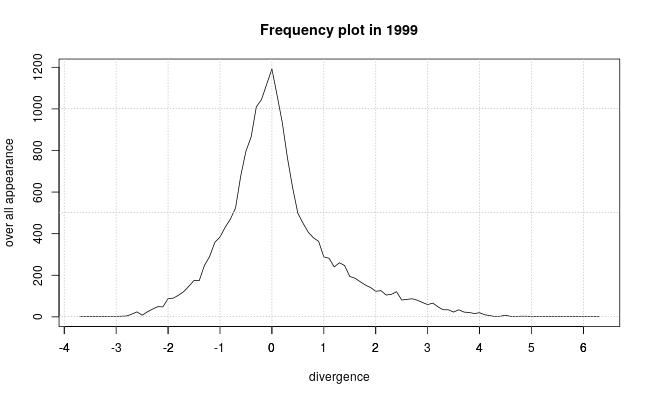
\includegraphics[width=\textwidth]{mean/ALP3/1999frequenciesdif_mprs_alp3eval-apgd.jpg}
		\caption{Absolute Häufigkeit der jährlich gemittelten Differenzen über das gesamt Gitter für das Jahr 1999 [mm/day]}
		\label{fig:freq_dif_eval_apgd_1999}
	\end{subfigure}
	\begin{subfigure}{\textwidth}
		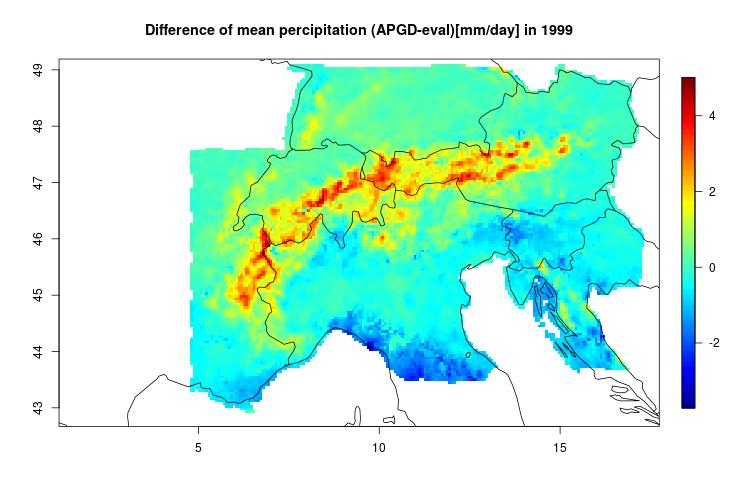
\includegraphics[width=\textwidth]{mean/ALP3/1999dif_mprs_alp3eval-apgd-cropped.jpg}
		\caption{Gemittelte Differenzen[mm/day] im Jahr 1999 für den evaluation-Datensatz mit ausgeschnittenem Ausreißer-Bereich}
		\label{fig:cropped_dif_eval_apgd_1999}
	\end{subfigure}
	\caption{Jährlich gemittelte Differenzen des Niederschlags im Jahr 1999 der evaluation Daten mit den APGD-Daten}
	\label{fig:eval_apgd}
\end{figure}
\\
Zu den Abbildungen in \ref{fig:eval_apgd}: in \ref{fig:dif_eval_apgd_1999} ist wieder ein Ausreißer-Bereich am südöstlichen Rand des Gitter zu erkennen, da dort eine überdurchschnittliche Abweichung herrscht, wurde dieser für die Berechnung der absoluten Häufigkeit ausgeschnitten, in Abb. \ref{fig:cropped_dif_eval_apgd_1999} ist schließlich der Ausreißer-Bereich entfernt worden und man erkennt eine großflächige Übereinstimmung mit den Beobachtungsdaten: selbst die Abweichungen im Gebirge des Alpenhauptkammes überschreiten kaum die 4mm/Tag - Marke, was sich auch in der gemittelten Differenz von $0.1357$ abzeichnet (im Vergleich dazu die Abweichung beim EUR-11 Datensatz : $0.1009$, in welchem jedoch die maximalen Abweichungen über 8mm/Tag hinausreichen (vgl. Abb. \ref{fig:eval_dif}))\\
\\
Im Folgenden soll analog zum EUR-11-Datensatz die Differenz über alle Jahre gemittelt bzw das 90. Quantil dieser Differenzen betrachtet werden um eine Allgemein-Aussage treffen zu können.\\
\begin{figure}[hbt!]
	\begin{subfigure}{0.49\textwidth}
		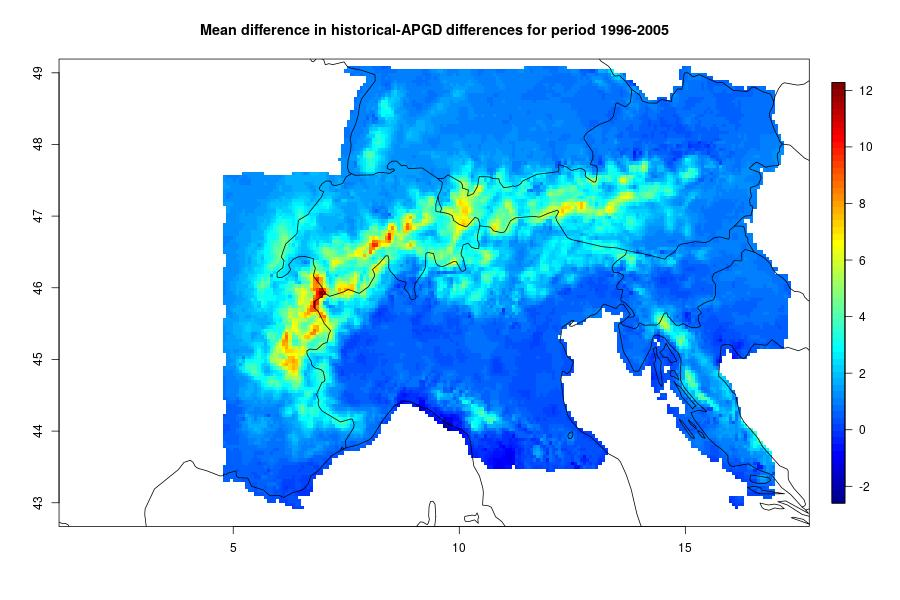
\includegraphics[width=\textwidth]{mean/ALP3/dif_mean_hist_apgd.jpg}
		\caption{Gemittelte Differenz[mm/day] für die Periode 1996-2005 des historical-Datensatzes}
		\label{fig:dif_hist_apgd_mean}
	\end{subfigure}
	\begin{subfigure}{0.49\textwidth}
		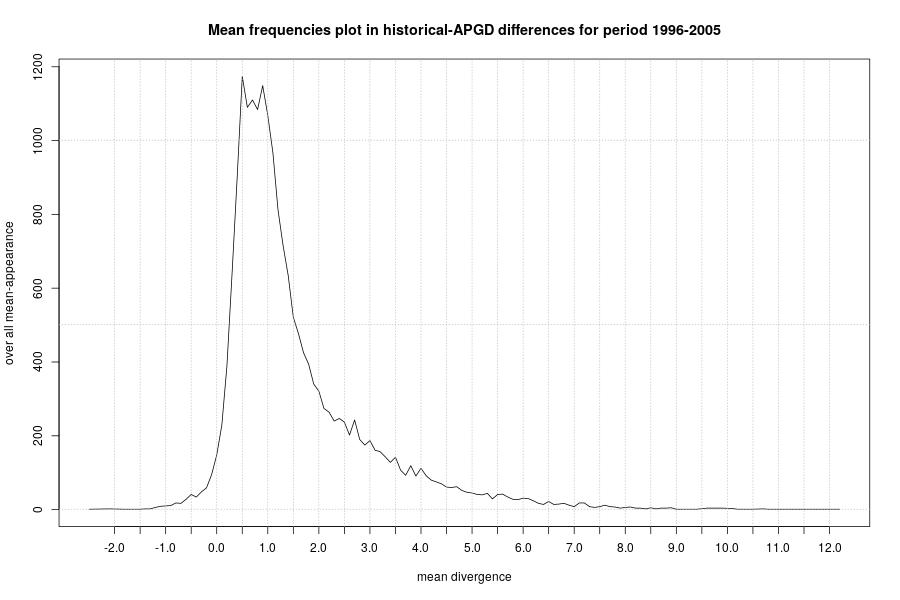
\includegraphics[width=\textwidth]{mean/ALP3/frequenciesdif_mean_hist_apgd.jpg}
		\caption{Absolute Häufigkeit der jährlich gemittelten Differenzen über das gesamt Gitter für die Periode 1996-2005}
		\label{fig:freq_dif_hist_apgd_mean}
	\end{subfigure}
	\begin{subfigure}{0.49\textwidth}
		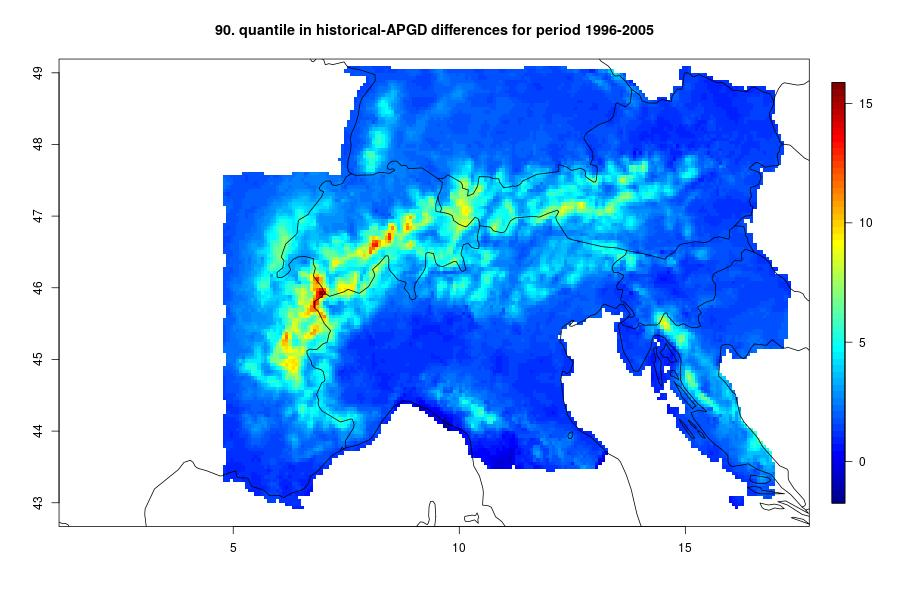
\includegraphics[width=\textwidth]{mean/ALP3/dif_q90_hist_apgd.jpg}
		\caption{90.Quantil der jährlich gemittelten Differenzen[mm/day] in der Periode 1996-2005 des historical-Datensatzes}
		\label{fig:dif_hist_apgd_q90}
	\end{subfigure}
	\begin{subfigure}{0.49\textwidth}
		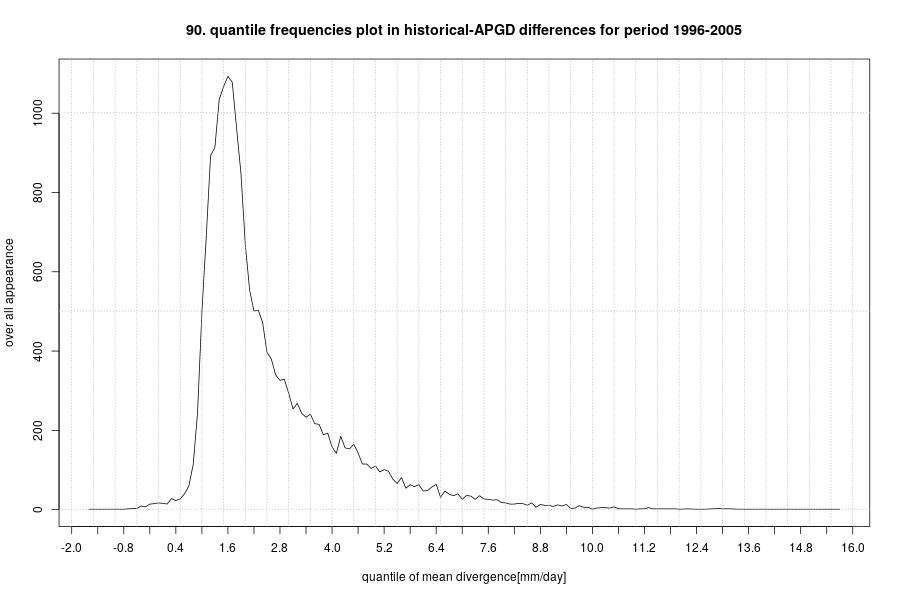
\includegraphics[width=\textwidth]{mean/ALP3/frequenciesdif_q90_hist_apgd.jpg}
		\caption{Absolute Häufigkeit des 90. Quantils der jährlich gemittelten Differenzen über das gesamt Gitter für die Periode 1996-2005}
		\label{fig:freq_dif_hist_apgd_q90}
	\end{subfigure}
	\caption{Differenzen des Niederschlags über die Periode 1996-2005 des historical-Datensatzes}
	\label{fig:mean_apgd_hist}
\end{figure}
\\
Man erkennt gut in Abb. \ref{fig:dif_hist_apgd_mean} und \ref{fig:dif_hist_apgd_q90}, dass die Niederschlagsmuster über den Alpen stark ins positive verzogen sind - zu starke Niederschläge wurden simuliert. Auch über der Ostküste des Mittelmeers sind die Niederschläge zu stark simuliert. Besonders zu beachten ist auch, der Verlauf der Kurve in Abb. \ref{fig:freq_dif_hist_apgd_mean} und \ref{fig:freq_dif_hist_apgd_q90} die klar ersichtlich macht, dass die Differenzen nahezu kaum ins Negative gehen und die Kurve stark bei $0$ ansteigt. Der Mittelwert der Differenzen über alle Jahre für den Datensatz historical beträgt $1.5583$, was verglichen mit dem Mittelwert der EUR-11-Differenzen von $0.5568$ einen überaus starken Zuwachs an Fehlern abbildet.\\
\begin{figure}[hbt!]
	\begin{subfigure}{0.49\textwidth}
		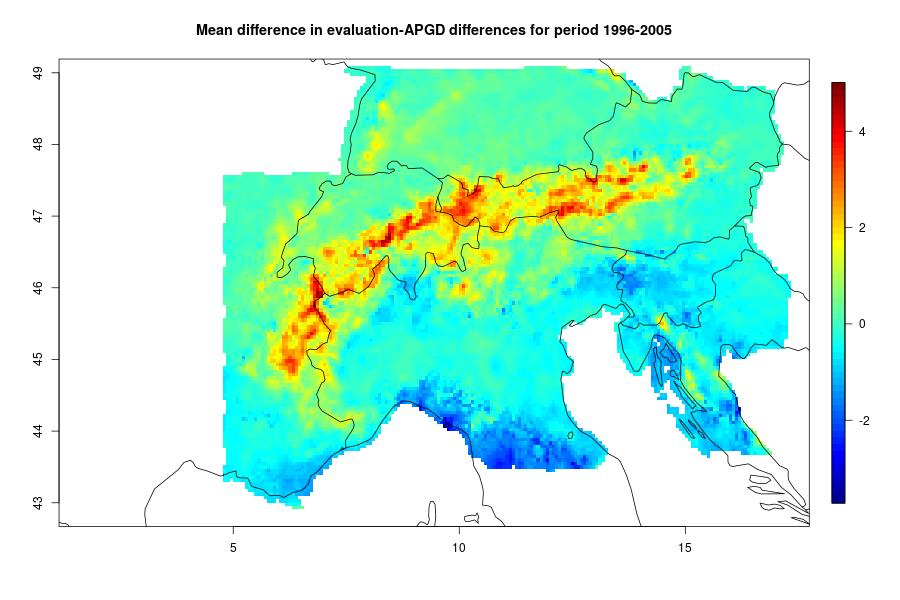
\includegraphics[width=\textwidth]{mean/ALP3/dif_mean_eval_apgd.jpg}
		\caption{Gemittelte Differenz[mm/day] für die Periode 1996-2005 des evaluation-Datensatzes}
		\label{fig:dif_eval_apgd_mean}
	\end{subfigure}
	\begin{subfigure}{0.49\textwidth}
		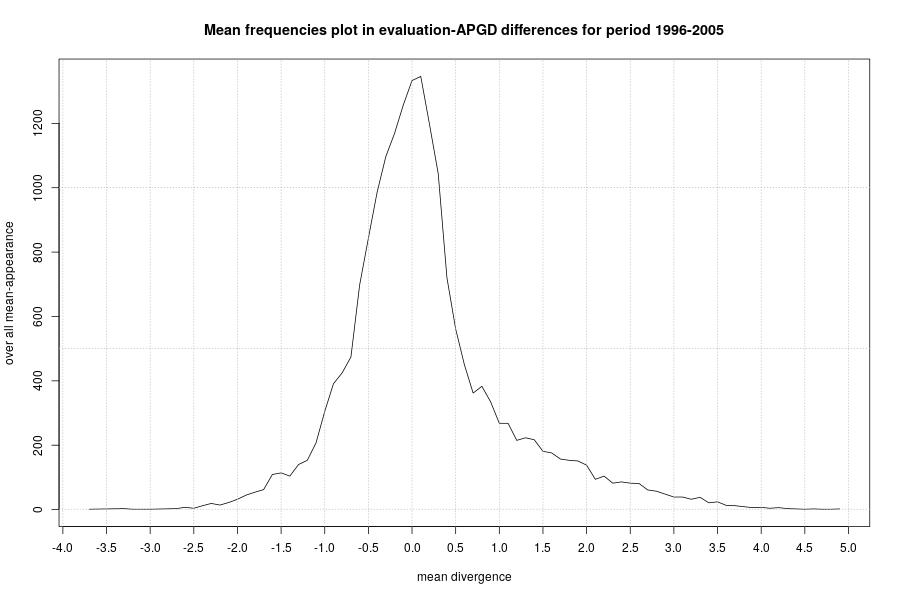
\includegraphics[width=\textwidth]{mean/ALP3/frequenciesdif_mean_eval_apgd.jpg}
		\caption{Absolute Häufigkeit der jährlich gemittelten Differenzen über das gesamt Gitter für die Periode 1996-2005}
		\label{fig:freq_dif_eval_apgd_mean}
	\end{subfigure}
	\begin{subfigure}{0.49\textwidth}
		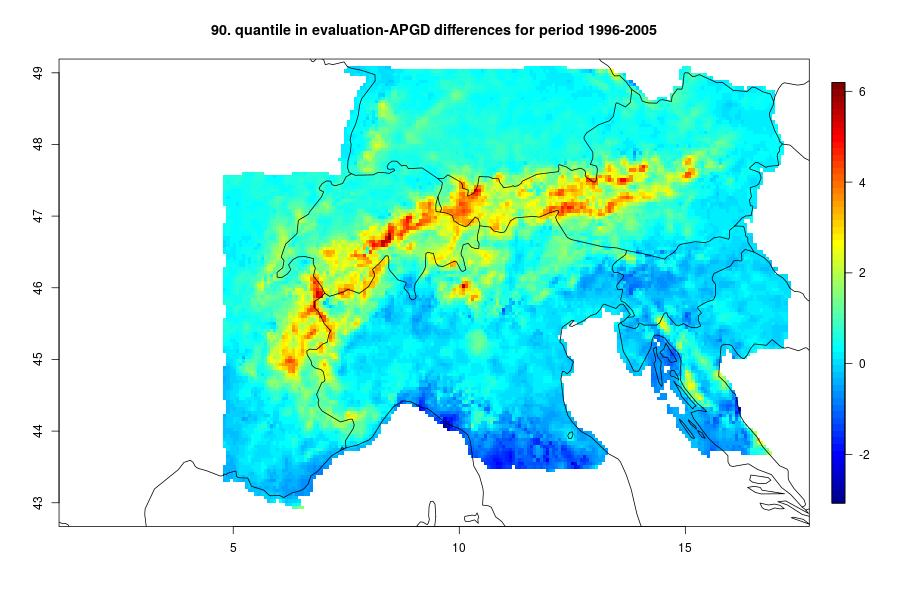
\includegraphics[width=\textwidth]{mean/ALP3/dif_q90_eval_apgd.jpg}
		\caption{90.Quantil der jährlich gemittelten Differenzen[mm/day] in der Periode 1996-2005 des evaluation-Datensatzes}
		\label{fig:dif_eval_apgd_q90}
	\end{subfigure}  
	\begin{subfigure}{0.49\textwidth}
		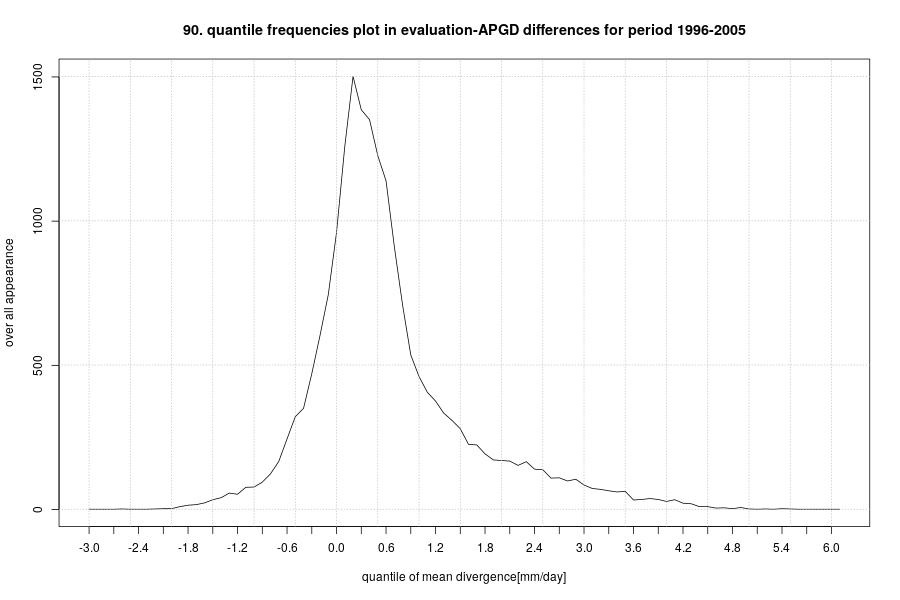
\includegraphics[width=\textwidth]{mean/ALP3/frequenciesdif_q90_eval_apgd.jpg}
		\caption{Absolute Häufigkeit des 90. Quantils der jährlich gemittelten Differenzen über das gesamt Gitter für die Periode 1996-2005}
		\label{fig:freq_dif_eval_apgd_q90}
	\end{subfigure}
	\caption{Differenzen des Niederschlags über die Periode 1996-2005 des evaluation-Datensatzes}
	\label{fig:mean_apgd_eval}
\end{figure}
\\
Die Berechnungen im evaluation-Datensatz scheinen ein um einiges besseres Ergebnis zu generieren als die des historical-Datensatzes (vgl. dazu Abb.\ref{fig:dif_eval_apgd_mean} und \ref{fig:dif_eval_apgd_q90}) die größte Abweichung im 99. Quantil beträgt $6.184$ und über der Mittelwert der Differenzen über alle Jahre gemittelt beträgt $0.1612$ was ungefähr der mittleren Abweichung im EUR-11 Datensatz entspricht: $0.1297$. Sie liegt zudem wie auch schon zuvor bei den EUR-11 Daten beobachtet über dem Mittelwert vom Jahr 1999 $0.1357$.\\
\vfill
\pagebreak[4]
\hfill
\vfill
\pagebreak[4]
\hfill
\vfill
\pagebreak[4]
\vfill
\section{Zusammenfassung}
\begin{table}[hbt!]
	\begin{tabu}to \textwidth{|X[2]|X|X|X|X|}
		\hline
		Typus& \textbf{EUR-11 historical} & \textbf{EUR-11 evaluation} &\textbf{ALP-3 hisstorical} & \textbf{ALP-3 evaluation}\\[0.2mm]
		\hline
		mW(M.d.D.(1999)) &$+0.4590$& $+0.1009$ &$+0.8304$& $+0.1612$\\
		\hline
		mW(M.d.D.(g.P)). &$+0.5568$ &$+0.1297$&$+1.5583$&$+0.1612$\\
		\hline
		max(M.d.D.(g.P))& $+10.8842$ & $+9.7163$ &$12.1646$ &$+4.9447$\\
		\hline
		min(M.d.D.(g.P))& $-2.6776$  &$-2.8346$  &$-2.4807$ &$-3.6535$\\
		\hline
		max(Q90(g.P)) & $13.7059$ & $13.3413$ & $15.7433$ & $6.1232$\\
		\hline
		min(Q90(g.P)) & $-2.0376$ & $-2.2838$ & $-1.6056$ & $-3.0018$\\
		\hline
	\end{tabu}
	\caption{Zahlenwerte der mittleren Abweichung\\M.d.D. ... Mittelwerte der Differenzen; \\g.P. ... gesamte Periode (1996-2005) bzw. für EUR-11 historical 1995-2005;\\mW ... Mittelwert\\Q90 ... 90.Quantile der jährlichen Mittelwerte über die gesamte Periode}
	\label{tab:Mean_Values}
\end{table}
Wie man in Tabelle \ref{tab:Mean_Values} sehen kann, sticht die ALP3-Simulation mit Evaluation-Daten betrieben als bestes Ergebnis hervor. Dies ist nicht überraschend, da das downscaling in diesem Fall mit konvektionserlaubender Simulation betrieben und mit Re-Analysedaten gefüttert wurde. Überraschend sind die bedeutend höheren Abweichungs-Werte des ALP3 historical Datensatzes der um einiges schlechter abschneidet wie der historical Datensatz im EUR-11. Die Zahlen des EUR-11 evaluation und historical - Datensatzes ähneln sich abgesehen vom Mittelwert über die Mittelwerte der gesamten Periode sehr, da durch das relativ große Gitter die Orthographie im Mittel nicht so stark ins Gewicht fällt- es gehen die Extremwert unter.
Bisher wurden die jährlichen Mittelwerte betrachtet, um die allgemeine Übereinstimmung der Daten zu betrachten, dies war für den evaluation Datensatz gegeben. Der historical Datensatz zeigt eine starke Abweichung von den Beobachtungsdaten. Um zu zeigen, wie sich eine Korrektion des Datensatzes über die Mittelwerte einer Beobachteten Periode auswirkt habe ich die das Jahr 1999 mit den Mittelwerten der gesamten Periode korrigiert, da die Ergebnisse mit den Abbildungen \ref{fig:dif_eval_apgd_1999} und \ref{fig:dif_hist_apgd_1999} gut zu vergleichen sind.
Das Ergebnis der Mittelwert-Korrektion findet man in Abb. \ref{fig:dif_new_1999}. Man erkennt in Abb.\ref{fig:dif_new_1999}, dass die Abweichung beinahe $0$ beträgt, auch über den Alpen hat die Abweichung einen Wert zwischen $0$ und $-2$. Die höchste Häufigkeit des liegt nun zwar leicht im negativen, mit einer mittleren Abweichung $-0.7292$


\begin{figure}[hbt!]
	\begin{subfigure}{0.49\textwidth}
			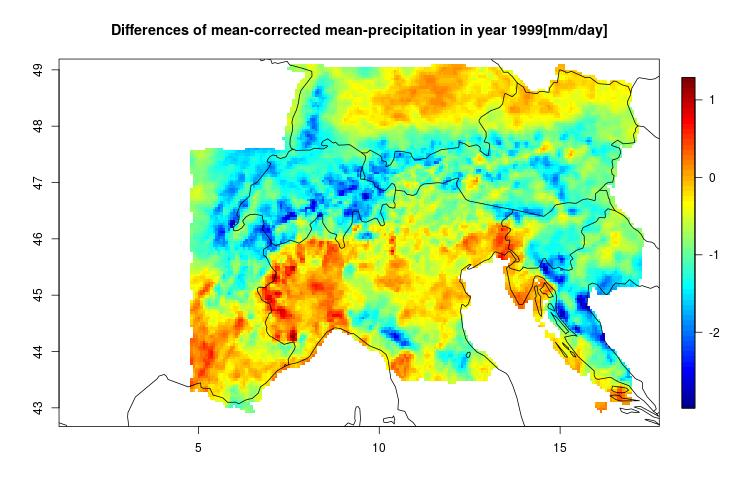
\includegraphics[width=\textwidth]{mean/ALP3/dif_new_1999.jpg}
		\caption{Differenzen des Mittelwert-korrigierten Jahres 1999 von den APGD-Daten (Simuliert-Beobachtet)}
		\label{fig:dif_new_1999}
	\end{subfigure}
	\begin{subfigure}{0.49\textwidth}
		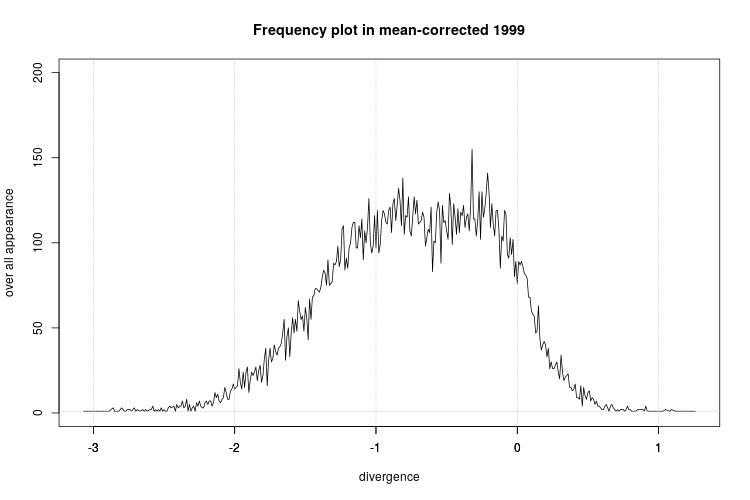
\includegraphics[width=\textwidth]{mean/ALP3/dif_new_1999_freq.jpg}
		\caption{Häufigkeit der Differenzen des Mittelwert-korrigierten Jahres 1999 von den APGD-Daten}
		\label{fig:dif_new_1999_freq}
	\end{subfigure}
\caption{Ergebnisse der Mittelwert-Korrigierten mittleren Niederschläge des Jahre 1999}
\end{figure}
